\section{Failure}

In a large-scale distributed stream processing system, failure should not be considered a rare, transient
condition. The previous section described failure due to overload (\ie when the system resources are
insufficient to carry out perfect processing). Failure, however, can also occur for other reasons.
When dealing with a large number of processing units, it is not uncommon for a node to crash, thus leading to
the partial disconnection of the query graph. It is also possible that a processing node becomes
temporarily unreachable because of a network partition, especially in a widely geographically distributed processing
infrastructure. 

A stream processing system should address such issues in order to achieve a high level of dependability.
The term dependability~\cite{dependability} in this context refers to the ability of a system to
withstand failure and to efficiently recover from it. It should choose an appropriate \emph{consistency
model}, a contract with the user stating how failure will be handled, and employ a \emph{replication
model} to be more resilient to the occurrence of failure.

\subsection*{Consistency Model}
When failure occurs in a stream processing system, a choice arises between stopping the delivery of
results while recovering or delivering incorrect results. In the first case, the \emph{availability} of
the system is reduced because no results are produced during the recovery phase; in the latter case it
is the \emph{consistency} of results that is compromised. The system can also opt for a hybrid
approach~\cite{availability-consistency} delivering first imperfect results, marking them as
``unstable'', while trying to correct them as soon as the failure has been overcome. This model is called
\emph{eventual consistency} because eventually all the delivered results will be correct.
Another approach, called \emph{relaxed consistency} is to avoid correcting results and instead trying to
augment them with a metric quantifying the amount of failure incurred~\cite{dependable-is-sensing}.
This approach has been adopted in this thesis because we consider failure a constant
operating condition of the system and the cost to achieve eventual consistency would become too high to
be acceptable.
			
Borealis~\cite{borealis-fault_tolerance} adopts a strict consistency model that aims at eventual
consistency. This means that in the case of tuple loss or misordering, the system tries to obtain
the correct final result. It achieves this by marking a stream on which an error has
occurred as \emph{tentative}.  Later the system attempts to restore the correct result by employing
a revision process, which ensures that the final result is correct.  Of course, this assumes a
scenario in which a fault is more an exception than the rule, as the cost for the revision process can
become high. There is no mechanism to quantify the input of the fault to the user. As the fault is
thought to be transient and recoverable the only feedback given to the user is that the stream content is
invalid and cannot be trusted until recovery. Instead, we propose a quality-centric data model that
allows the system to quantify the impact of the error and to provide the user with feedback on the
actual processing quality of the system.\\
The revision mechanism used in Borealis also supports ``time travel''.  It is possible to recalculate
tuples for the past and even in the future (by providing a prediction formula).
Rolling back processing to the past is a heavy-weight process and requires a large
amount of storage, which is not always feasible in stream processing.\\
Figure~\ref{fig:borealis-fault_tolerance} shows the state machine for the fault tolerance mechanism
employed by Borealis. When failure occurs upstream in the query graph, an operator is alerted by the
arrival of tentative tuples or by the lack of heartbeat messages.
It then marks its tuples as tentative while waiting the restoring of a stable
state for the processing. When failure has been overcome, the state is reconciled and the system
becomes stable once again.

\begin{figure}[t] 
	\centering
	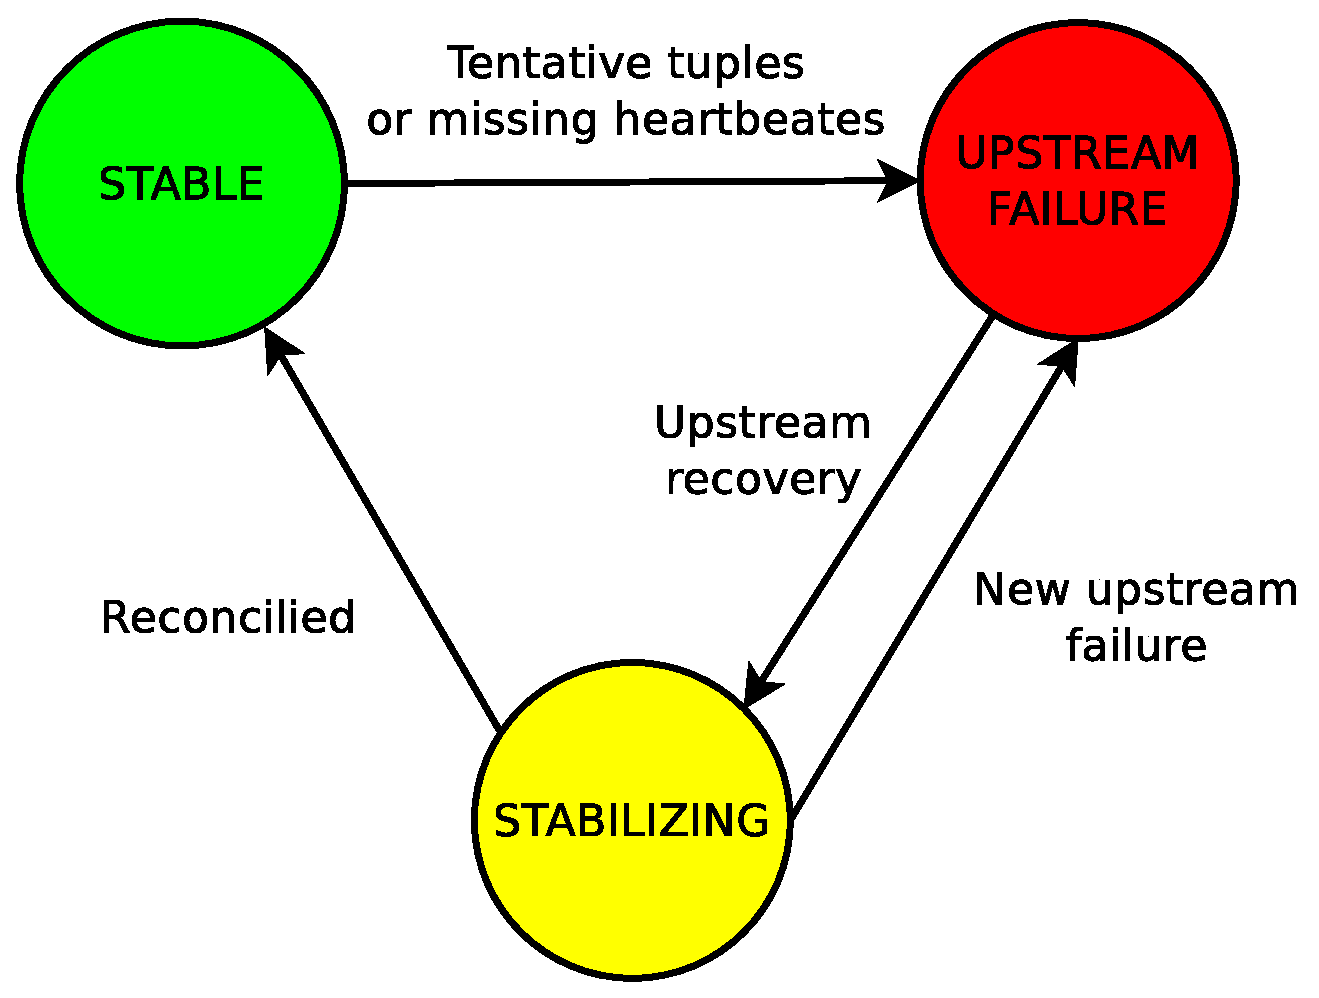
\includegraphics[width=.4\textwidth]{img/tesi/borealis-fault_tolerance}
	\caption{State machine describing Borealis fault tolerance mechanism in Borealis. }
\label{fig:borealis-fault_tolerance}
\end{figure}

In the relax consistency model proposed by Murty and Welsh~\cite{dependable-is-sensing}, operators are
considered to be \emph{free-running}, updating their internal state independently as incoming tuples
arrive. This means that two replicas of the same operator may produce different outputs because of their
different internal state due to failure.
Instead of trying to achieve eventual consistency, they propose to
deliver imperfect results but augmenting them with two quality metrics called \emph{harvest} and
\emph{freshness}. These metrics provide the user with information about the quality of the results.
Harvest represents the coverage of a query result in terms of data sources. Its value is reduced by
failures during query processing. A harvest of 100\% indicates that the result was computed
using data from all sources.
This metric is not directly related to correctness but rather provides an indication of
the confidence the user should have in the delivered results. A high value for harvest means that
the provided result incorporates a large number of the input sources.
Freshness represents the age of the input data that generated the result. A high network latency or a
high system load affect the freshness value of the delivered tuples negatively. The lower bound for
freshness is the network latency.

	
\subsection*{Replication Models}

In order to be more resilient to failure, stream processing systems frequently employs \emph{operator
replication}.
The system identifies the most important operators in a query and runs multiple copies of them
concurrently.
In this way, if a node hosting a part of the query fails, one of its replicas can be used instead,
without any impact on the processing.
Replication is not only useful to increase the dependability of the system but it can also improve its
performance by running the replicas in competition in order to reduce
latency~\cite{borealis-fast_and_ha, borealis-fast_and_reliable}.

%borealis
Early work on replication in a DSPS have been focused on masking software
failures~\cite{borealis_ha_algos} by running multiple copies of the same operators at different nodes.
Others~\cite{ha_ft_dataflows} proposed to strictly favour consistency over availability by
requiring at least one fully connected copy of the query graph to be working correctly in order for the
computation to proceed. %\\
In Borealis, the approach has been to provide a configurable trade-off between availability and
consistency~\cite{borealis-fault_tolerance}.
This is done by letting the user specify a time threshold, within which all tuples are processed
regardless of whether failures occurred or not on the input streams. This increases availability because
the operator continues to process even in the presence of failures on its input streams. Output tuples,
are then marked as \textit{tentative} in order to signal the incorrectness of the results. After the
system has recovered from the failure, it reconciles the state of operators that processed
tentative tuples, by re-running their computation with the stable data tuples. This also means that every
source or operator has to buffer all their outgoing tuples, at least for a certain amount of time, to
replay them in case of failure. The goal of Borealis is to achieve \textit{eventual consistency} and
provide all clients with complete correct results.

%murty&welsh
Another approach to the management of replicas has been proposed in~\cite{dependable-is-sensing}. The authors take a
different standpoint on failure by not considering it as an infrequent event but as a constant condition
of the system. In this case, maintaining consistency among replicas becomes even harder. The
authors claim that it is better to ignore this requirement and to employ \textit{free-running} operators
instead.
Operators are permitted to update their internal states independently as incoming tuples arrive. In case
of recovery from failure, for example, an operator restarts, without any knowledge of its
previous state. However, this means that an operator's state can diverge from its replicas due to
missing tuples.
In general, though, the state of an operator is based only on the tuples in its \textit{causality
window}. Thus, assuming a window size of $w$ seconds and no additional failure, the system will regain
consistency without the need for explicit synchronization. Whenever the replicas are out of sync and
produce different results, however, the system needs to choose, which set of results represents the
``best'' answer.
It can do so in several ways, for example, by choosing tuples generated by the replica with the largest
uptime, with a majority vote among the replicas, or by relying on some \textit{quality metric}
describing the quality of the data. This process is referred to as \textit{best-guess reconciliation}.
